%% автогенерация: scripts/figures_tex.py — руками не править
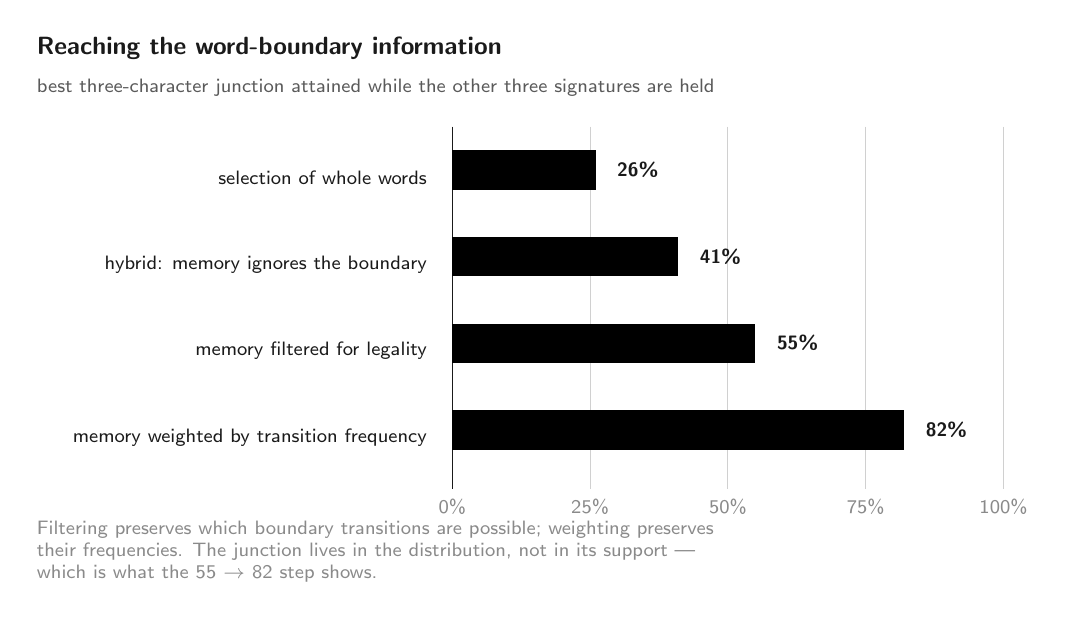
\begin{tikzpicture}[x=1mm,y=1mm,font=\sffamily\scriptsize]
\definecolor{ink}{HTML}{1A1A1A}\definecolor{inkii}{HTML}{5A5A5A}
\definecolor{inkiii}{HTML}{8A8A8A}\definecolor{rule}{HTML}{D0D0D0}
\definecolor{fill}{HTML}{2B2B2B}\definecolor{fillii}{HTML}{9A9A9A}
\definecolor{filliii}{HTML}{C8C8C8}
\node[anchor=west,font=\sffamily\small\bfseries,text=ink] at (0,57) {Reaching the word-boundary information};
\node[anchor=west,text=inkii] at (0,52) {best three-character junction attained while the other three signatures are held};
\draw[ink] (54.0,47) -- (54.0,1);
\node[below,text=inkiii] at (54.0,1) {0\%};
\draw[rule] (71.5,47) -- (71.5,1);
\node[below,text=inkiii] at (71.5,1) {25\%};
\draw[rule] (89.0,47) -- (89.0,1);
\node[below,text=inkiii] at (89.0,1) {50\%};
\draw[rule] (106.5,47) -- (106.5,1);
\node[below,text=inkiii] at (106.5,1) {75\%};
\draw[rule] (124.0,47) -- (124.0,1);
\node[below,text=inkiii] at (124.0,1) {100\%};
\node[anchor=east,text=ink] at (52,40.5) {selection of whole words};
\fill[fill] (54,39) rectangle (72.2,44);
\node[anchor=west,font=\sffamily\scriptsize\bfseries,text=ink] at (73.7,41.5) {26\%};
\node[anchor=east,text=ink] at (52,29.5) {hybrid: memory ignores the boundary};
\fill[fill] (54,28) rectangle (82.7,33);
\node[anchor=west,font=\sffamily\scriptsize\bfseries,text=ink] at (84.2,30.5) {41\%};
\node[anchor=east,text=ink] at (52,18.5) {memory filtered for legality};
\fill[fill] (54,17) rectangle (92.5,22);
\node[anchor=west,font=\sffamily\scriptsize\bfseries,text=ink] at (94.0,19.5) {55\%};
\node[anchor=east,text=ink] at (52,7.5) {memory weighted by transition frequency};
\fill[fill] (54,6) rectangle (111.4,11);
\node[anchor=west,font=\sffamily\scriptsize\bfseries,text=ink] at (112.9,8.5) {82\%};
\node[anchor=west,text=inkiii,align=left] at (0,-7) {Filtering preserves which boundary transitions are possible; weighting preserves\\their frequencies. The junction lives in the distribution, not in its support ---\\which is what the 55 $\to$ 82 step shows.};
\end{tikzpicture}
